\documentclass{anschreiben}

\renewcommand{\deinName}{Ingo Blechschmidt und Rolf Wittmann}
\renewcommand{\deineMailAdresse}{iblech@speicherleck.de und rkw95@web.de}


\renewcommand{\datum}{\today}
\renewcommand{\betreff}{Matheschülerzirkel der Universität Augsburg}

\begin{document}

\newread\quelle
\openin\quelle=teilnehmende.csv
\read\quelle to \zeile

\loop
\read\quelle to \zeile
\ifeof\quelle\global\morefalse\else

\bearbeitezeile

\ifganzeklasse Liebe Schülerinnen und Schüler,\else
\ifweiblich Liebe\else Lieber\fi{} \vorname,\fi

es ist endlich soweit, mit diesem Brief beginnt der Korrespondenzzirkel.

Wir möchten euch Zirkelteilnehmende über das Schuljahr verteilt auf eine
Rundreise durch ganz verschiedene Ecken der Mathematik mitnehmen. Für
Themenwünsche sind wir immer offen! Wenn ihr etwa etwas Interessantes auf
Wikipedia entdeckt habt und dazu gerne mehr wissen möchtet, dann meldet euch
einfach bei uns.

Wir sind Ingo und Rolf, eure Zirkelleiter. Rolf studiert im Master und Ingo hat
vor ein paar Wochen seine Promotion in Mathematik abgeschlossen. Wenn ihr uns
E-Mails schreibt, dann duzt uns einfach und gebt euch keine Mühe, besonders
höfliche Formulierungen aufzusetzen. Wir sind nur Studenten und freuen uns,
wenn ihr uns auch so behandelt. :-)

Anbei der erste Brief. Es geht um Spieltheorie! Das ist einerseits ein
Teilgebiet der angewandten Mathematik, wenn man etwa Handlungsoptionen für
Unternehmen oder Staaten analysiert. Andererseits gehört es auch zur reinen
Mathematik. Es bestehen nämlich ganz wundersame Beziehungen zum Studium der
unendlich großen Zahlen (diejenigen Zahlen, die auf einem erweiterten
Zahlenstrahl nach den in der Schule behandelten Zahlen kommen -- wenn ihr euch
einen Zirkel zu diesen Zahlen und anderen Phänomenen des Unendlichen wünscht,
gebt Bescheid).

Mathematik ist kein Sport für bloße Zuschauerinnen und Zuschauer; man lernt
Mathematik nur, wenn man sich lange Zeit mit Übungsaufgaben beschäftigt. Aus
diesem Grund habt ihr beim Korrespondenzzirkel die Möglichkeit, die in den Text
integrierten Aufgaben zu bearbeiten und eure Lösungsideen an uns zu schicken
(per Mail oder Post, wie es euch besser gefällt). Wer bis zum 30. November
seine Lösungen einschickt, erhält von uns eine ausführliche Korrektur.

Wir wünschen euch viel Spaß mit dem ersten Korrespondenzbrief! Bitte zögert
keine Sekunde, euch bei Fragen aller Art an uns zu wenden. An der Uni sind die
besten Seminare die, die es schaffen, eine gründliche Fragekultur zu
etablieren, bei der sich jeder wohlfühlt, auch vermeintlich einfache Fragen zu
stellen. Wir hoffen, dass wir eine solche Atmosphäre auch hier etablieren
können. Fragt also immer nach, wenn ihr gerade irgendwo hängt. Das können auch
ganz offene Fragen wie "`erklärt doch bitte noch mal genauer, was ihr mit XX
meint"' sein.

\enlargethispage{2em}
Viele Grüße

Ingo und Rolf

PS: Der nächste Korrespondenzbrief wird den Pentagonalsatz aus der Kombinatorik
und Zahlentheorie behandeln.

PPS: Wir sind große Fans vom Numberphile-Kanal auf YouTube. (Zu seiner
Unterstützung überweisen wir jeden Monat $\tau$ Dollar an die Macher.) Falls
ihr ihn noch nicht kennt, dann schaut euch unbedingt mal ein paar Videos an.
(Was ist euer Lieblings-Mathe-Kanal auf YouTube? Bitte sagt es uns!)

PPPS: Vor kurzem ist viel zu früh Maryam Mirzakhani verstorben, eine großartige
Mathematikerin, die für ihre Arbeiten 2014 mit der Fields-Medaille (für viele
die höchste Auszeichnung in der Mathematik) geehrt wurde. Wer etwas zu
Mirzakhani als Person oder zu ihren Forschungsgebieten erfahren möchte, kann
sich einen Artikel des Quanta Magazine ansehen: https://tiny.cc/iybtoy

\begin{center}
  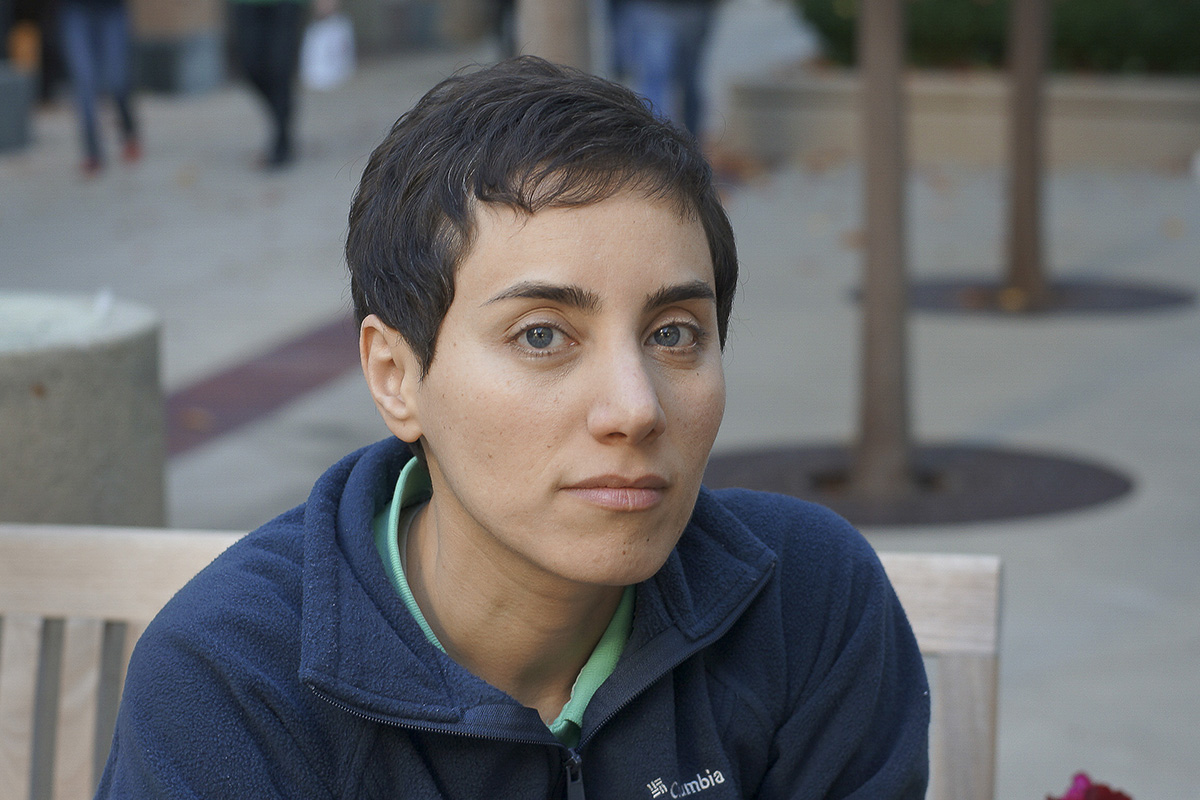
\includegraphics[width=0.6\textwidth]{mirzakhani}
\end{center}

\newpage
\fi\ifmore\repeat

\closein\quelle

\end{document}
